\subsection{Algorithme de Dowek}

\subsubsection{Precooking}

En $\lambda\sigma$-calcul, les opérations grafting et de réduction commutent. C'est pour cette raison que l'on peut utiliser le grafting dans l'unification higher-order du \lsc{}. En effet l'unification dans le \lsc{} calcule un grafting qui rends les termes égaux, tandis que l'unification dans le lambda-calcul calcule une substitution. Pour réaliser l'unification higher-order, on souhaite travailler avec des graftings.

Pour réaliser l'unification dans le \lc{}, on va traduire les termes du \lc{} vers le \lsc{}, cette opération est nommée precooking :

\begin{defn}
Soit $a \in \Lambda_{DB}(X)$ tel que $\Gamma \vdash a\ :\ T$. Pour chaque variable $X$ de type $U$ dans le terme $a$, on associe le type $U$ dans le contexte $\Gamma$ dans le \lsc{}. Le precooking de $a$ depuis le \lc{} vers le \lsc{} est défini par $a_F = F(a, 0)$ où $F(a, n)$ est :

\begin{enumerate}
    \item $F((\lambda_B a), n) = \lambda_B(F(a, n + 1))$
    \item $F(k, n) = 1[\uparrow^{k-1}]$
    \item $F((a b), n) = F(a, n) F(b, n)$
    \item $F(X, n) = X[\uparrow^n]$
\end{enumerate}

\end{defn}

\subsubsection{Algorithme d'unification}

Nous allons présenter l'algorithme d'unification utilisé dans le papier de Dowek \cite{dowek1995higher}. Comme dit précédemment, une solution est un grafting des métavariables vers les termes.

D'un point de vus formelle on cherche à appliquer des règles d'unification (présentées \hyperref[unificationrules]{plus tard}) sur un système d'équations. Nous avons dû faire un choix afin de représenter cela dans notre système. Voici les différentes structures que nous avons définies :

\begin{lstlisting}
type equa = 
  | DecEq of s_term * s_term
  | Exp

type and_list = equa list

type unif_rules_ret =
  | Ret of (and_list * meta_var_str) list
  | Rep of name * s_term * and_list
  | Nope
  | Fail
\end{lstlisting}

Le type \verb|equa| permet de représenter les équations. Nous avons besoin d'un cas \verb|exp| qui sera utilisé par notre fonction d'unification pour traiter le cas où il n'y a plus aucunes équations sur lesquelles appliquer des règles, nous y reviendrons plus tard.

Le type \verb|and_list| nous permet de représenter les 
disjonctions du système d'équations.
Et enfin le type \verb|unif_rules_ret| est notre type de retour personnalisé pour l'algorithme d'unification.
Avant d'expliquer ce type, il est important de parler de l'architecture des fonctions que nous avons définies pour l'unification.
\begin{figure}[H]
    \centering
    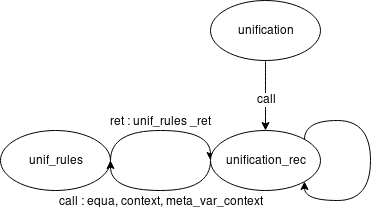
\includegraphics[scale=0.6]{images/unif_diagram.png}
\end{figure}

Étant donné que certaines règles peuvent produire de nouveaux systèmes d'équations étant d'autres solutions potentielles
le constructeur \verb|Ret| retourne des listes de solutions.
Le constructeur \verb|Replace| permet de notifier que la règle doit être suivie d'un remplacement, le \verb|Nope| notifie que l'on n'a pas trouvé de pattern dans l'équation permettant de trouver. \verb|Fail| notifie que l'on a trouver une contradiction.


Présentons maintenant l'ensemble des règles d'unification (pour chaque règle on présente la partie formelle et l'implémentation) :\label{unificationrules}

\textbf{Dec-$\lambda$} :
\begin{align*}
    &P \wedge \lambda_A a =_{\lambda \sigma}^{?} \lambda_A b \\
    &\xrightarrow{} \\
    &P \wedge a =_{\lambda \sigma}^{?} b
\end{align*}
Cette règle permet simplement de rentrer sous les $\lambda$ si les deux termes de l'équation sont des abstractions.

\begin{lstlisting}[frame=single]
| DecEq (S_Abs (typ1, t1), S_Abs (typ2, t2)) -> 
    if eq_typ typ1 typ2 then Ret [([ DecEq (t1, t2)], ctx)] else Fail
\end{lstlisting}

\textbf{Dec-App} :
\begin{align*}
    &P \wedge (n \, a_1 \dots a_p) =_{\lambda \sigma}^{?} (n \, b_1 \dots b_p) \\
    &\xrightarrow{} \\
    &P \wedge (\wedge_{i=1 \dots p} a_i =_{\lambda \sigma}^{?} b_i)
\end{align*}
Cette règle crée de nouvelles équations entre chacun des arguments. Il est à noter qu'avec notre représentation nous ne possédons pas d'applications à plusieurs arguments, nous n'avons donc pas à traiter ce cas général mais le sous-cas réduit à une seule application.
De plus, cette règle peut trouver une contradiction si les deux fonctions ne sont pas égales. Ce qui est traduit par la règle suivante :

\textbf{Dec-Fail} :
\begin{align*}
    &P \wedge (n \, a_1 \dots a_p) =_{\lambda \sigma}^{?} (m \, b_1 \dots b_q) \\
    &\xrightarrow{} \\
    &F \\
    &\text{si $n \neq m$}
\end{align*}

Ces deux cas sont gérer par notre implémentation dans le traitement du même pattern.
\begin{lstlisting}[frame=single]
  | DecEq (S_App (t1, t2), S_App (t3, t4)) ->
    if t1 = t3 then Ret [([DecEq (t2, t4)], ctx)]
      else Fail
\end{lstlisting}

\textbf{Replace} :
\begin{align*}
    &P \wedge X =_{\lambda \sigma}^{?} a \\
    &\xrightarrow{} \\
    &\{ X \mapsto a \} (P) \wedge X =_{\lambda \sigma}^{?} a \\
    &\text{si $X \in TVar(P)$, $X \notin TVar(a)$ et $a$ une métavariable $\implies a \in TVar(P)$}
\end{align*}

Le replace est une règle particulière car elle se contente simplement de remplacer une variable d'unification si celle-ci ne comporte pas de substitution. \E{}tant donné notre implémentation, nous ne pouvons pas effectuer ce traitement dans la fonction appliquant les règles directement. C'est pour cette raison que nous avons rajouté un constructeur \verb|Repl| dans le type \verb|unif_rules_ret|.
Grâce à cela, notre fonction principale sera à même d'effectuer ce remplacement. 

\begin{lstlisting}[frame=single]
(* REP *)
  | DecEq (S_Xvar (n), t) -> Rep (n, t, [e])
\end{lstlisting}

\textbf{Normalize} :
\begin{align*}
    &P \wedge a =_{\lambda \sigma}^{?} b \\
    &\xrightarrow{} \\
    &P \wedge a' =_{\lambda \sigma}^{?} b' \\
    &\text{si $a$ ou $b$ n'est pas une forme normale longue}\\
    &\text{$a'$ (resp. $b'$) est la forme normale longue de $a$ (resp. $b$) si $a$ (resp. $b$) n'est pas une variable résolue et $a$ (resp. $b$) sinon}
\end{align*}

De même que pour replace cette règle est un peu spéciale puisque étant donné que l'on souhaite travailler uniquement avec des termes normalisés nous nous assurons au cours de l'algorithme d'appeler la fonction de normalisation aux différents endroits où celle ci est nécessaire.

\textbf{Exp-App} :
\begin{align*}
    &P \wedge X[a_1 \dots a_p . \uparrow^n] =_{\lambda \sigma}^{?} (m \, b_1 \dots b_q) \\
    &\xrightarrow{} \\
    &P \wedge X[a_1 \dots a_p . \uparrow^n] =_{\lambda \sigma}^{?} (m \, b_1 \dots b_q) \\
    &\quad \wedge \vee_{r \in R_p \cup R_i} \exists H_1, \dots, H_k, X =_{\lambda \sigma}^{?} (r \, H_1 \dots H_k) \\
    &\text{si $X$ est un type atomique et n'est pas résolu} \\
    &\text{où $H_1, \dots , H_k$ sont des variables de types appropriés, qui n'apparaissent pas dans $P$, avec les contextes $\Gamma_{H_i} = \Gamma_X$, $R_p$ est un sous-ensemble de $\{ 1,\dots,p \}$ tel que $(r \, H_1 \dots H_k)$ a le bon type, $R_i=$ si $m \geq n+1$ then $\{m-n+p\}$ else $0$}
\end{align*}

Cette règle permet de supprimer les substitutions associées aux variables d'unification. Malgré son apparente complexité, le but de cette règle est de créer un ensemble de nouvelles solutions (ce qui va entraîner des appels récursifs à notre fonction d'unification).

\begin{lstlisting}[frame=single]
(* EXP APP *)
  | DecEq (S_Tsub (S_Xvar(x), s), t) ->
    let (typ, _) = Map_str.find x ctx in
    let lst = find_var_end_typ ct typ in
    create_disjunctions (S_Xvar (x)) ct ctx lst
\end{lstlisting}

\textbf{Exp-$\lambda$} :
\begin{align*}
    &P \\
    &\xrightarrow{} \\
    &\exists Y : (A . \Gamma \vdash B), \quad P \wedge X =_{\lambda \sigma}^{?} \lambda_A Y  \\
    &\text{si $(X : \Gamma \vdash A \xrightarrow{} B) \in TVar(P), Y \notin TVar(P)$, et $X$ n'est pas une variable résolue}
\end{align*}

Cette règle a pour but d'essayer de continuer l'unification lorsque plus aucune des règles précédentes ne sont applicables. C'est pour cette raison que nous avons rajouter le constructeur \verb|Exp| comme type pour les équations. Cela va donc forcer notre fonction à exécuter cette règle.
Celle-ci consiste à utiliser la \textit{$\eta$-expansion} sur une variable du contexte qui n'est pas résolue. Il faut également que cette variable ait un type \verb|arrow| (sinon il est impossible d'appliquer la \textit{$\eta$-expansion}).

Nous avons donc présenté l'ensemble des règles nécessaires à l'unification, voici maintenant la fonction \verb|unification_rec| : 
\newpage
\begin{lstlisting}
unification_rec (s: and_list) (su : (and_list * unif_rules_ret list)) (ctx : meta_var_str) (ct : context) : ((and_list * meta_var_str) list) option =
  if is_that_finished ctx then Some [(s,ctx)]
  else
    let (old_liste, ret_liste) = su in
    (match s with
     | [] -> (
        match look_res_list ret_liste with 
        | FullNope -> (
          match unif_rules Exp ct ctx with
          | Ret l -> start_unification_list l ct su
          | Rep (res_name,res_term,res_s) -> unification_rec (replace_and_list res_name res_term (old_liste @ res_s)) ([],[]) (put_metaVar_true res_name ctx) ct 
          | Nope -> None
          | Fail -> None)                           
        | OneRet -> unification_rec (fst su) ([],[]) ctx ct
        | Failed -> None)
    | a :: tl ->
      let (old_liste, ret_liste) = su in
      let ret = unif_rules a ct ctx in
      let new_su = (old_liste @ [a] ,ret_liste @ [ret]) in
      (match ret with  (* unification_rec tl new_su *)
        | Ret l -> start_unification_list l ct new_su
        | Rep (res_name,res_term,res_s) -> unification_rec (replace_and_list res_name res_term (old_liste @ res_s)) ([],[]) (put_metaVar_true res_name ctx) ct 
        | Nope -> None
        | Fail -> None))
\end{lstlisting}